\section{Laufzeitanalysen}
\begin{table}[b]
	\centering
	\begin{tabular}{ll}
		\hline \hline
		\vspace{-3mm}\\
		Prozessor		& 2x Intel Xeon CPU E5-2667 0 @ 2.90GHz\\
		Arbeitsspeicher	& 8x 16 GB DDR3 @ 1600MHz\\
		Grafikkarte		& 2x Nvidia Tesla K20c\\
		Hauptplatine	& Dell 0F5XM3\\
		\hline
	\end{tabular}
	\caption{Ausstattung des Testrechners}
	\label{table:systemausstattung}
\end{table}

Das System, auf dem der Algorithmus getestet wurde, ist in Tabelle \ref{table:systemausstattung} beschrieben.

Um die Performance des Extraktors zu messen und zu vergleichen wurde ein Shellscript geschrieben. Als Testparameter wurde $m$, die Anzahl der zu extrahierenden Bits, gew"ahlt, wobei $m = 2^M$ und $M \in \{8, \dots, 20\}$. Die gew"ahlte Seedl"ange $n$ ist immer um den Faktor $16$ gr"o"ser als $m$. Um den Einfluss einzelner Ausrei"ser zu mindern, wird der Test 18 mal wiederholt. Abbildung \ref{fig:laufzeitCpuGpu2} zeigt einen Plot der Ergebnisse des Tests, wobei der Median und das obere und untere Dezil betrachtet werden.


\begin{comment}
\begin{figure}
	\centering
	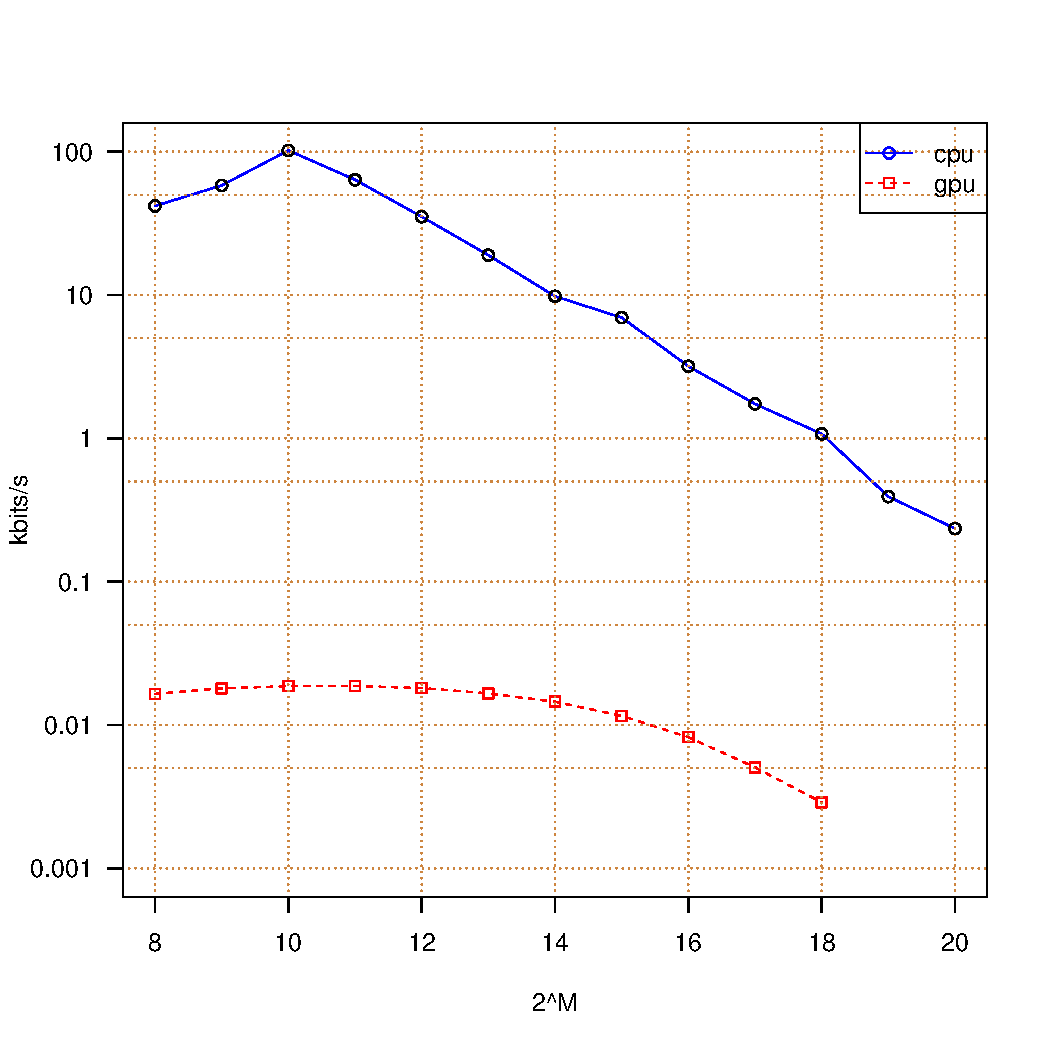
\includegraphics[scale=.5]{combined.pdf}
	\caption{Laufzeit CPU vs GPU}
	\label{fig:laufzeitCpuGpu}
\end{figure}
\end{comment}
\begin{figure}[h]
\centering
\begin{tikzpicture}[trim axis left,trim axis right]
\begin{axis} [ymode=log, xtick={8,10,12,14,16,18,20}, scale=1.5, grid=both, minor ytick={.005,.05,.5,5,50,500}, minor xtick={9,11,13,15,17,19}, legend entries={,CPU,,,,GPU},xlabel=$2^M$,ylabel={kbit/s [log. Skala]}]
    \addplot [box plot box] table {Bilder/output_rsh.dat};
    \addplot [box plot median] table {Bilder/output_rsh.dat};
    \addplot [box plot top whisker] table {Bilder/output_rsh.dat};
    \addplot [box plot bottom whisker] table {Bilder/output_rsh.dat};
    \addplot [box plot box] table {Bilder/output_rshCuda.dat};
    \addplot [box plot median, /pgfplots/other color] table {Bilder/output_rshCuda.dat};
    \addplot [box plot top whisker] table {Bilder/output_rshCuda.dat};
    \addplot [box plot bottom whisker] table {Bilder/output_rshCuda.dat};
\end{axis}
\end{tikzpicture}
\caption{Laufzeit CPU vs GPU \protect\\ \normalfont Die x-Achse des Liniendiagramms gibt die Anzahl der zu extrahierenden Bits an und \protect\\ die y-Achse zeigt die gemessene Performance in \emph{kbits/s} auf einer logarithmischen Skala.}
\label{fig:laufzeitCpuGpu2}
\end{figure}

Die beiden Testparameter $M=19$ und $M=20$ f"uhren in der aktuellen Implementierung zu Speicherzugriffsfehlern. Dies wurde w"ahrend des Entwickelns nicht deutlich, da aus Zeitgr"unden nur kleine Werte f"ur $m$ und $n$ getestet wurden (die Extraktion von $2^{18}$ Bits dauert ca. 30 Stunden).

Aus den gemessenen Werten geht hervor, dass der CPU-Algorithmus um den Faktor $10^3$ schneller ist als die GPU-Implementierung. Die Kurve des GPU-Algorithmus bleibt allerdings "uber einen gr"o"seren Wertebereich von $M$ stabil und beginnt erst bei $M=15$ vergleichbar stark abzunehmen wie der CPU-Algorithmus ab $M=10$. Da der GPU-Algorithmus einiges Potential zur Optimierung bietet, besteht die M"oglichkeit vergleichbare Extraktionsraten zu erzielen.
